% Created by tikzDevice version 0.11 on 2019-01-03 16:01:30
% !TEX encoding = UTF-8 Unicode
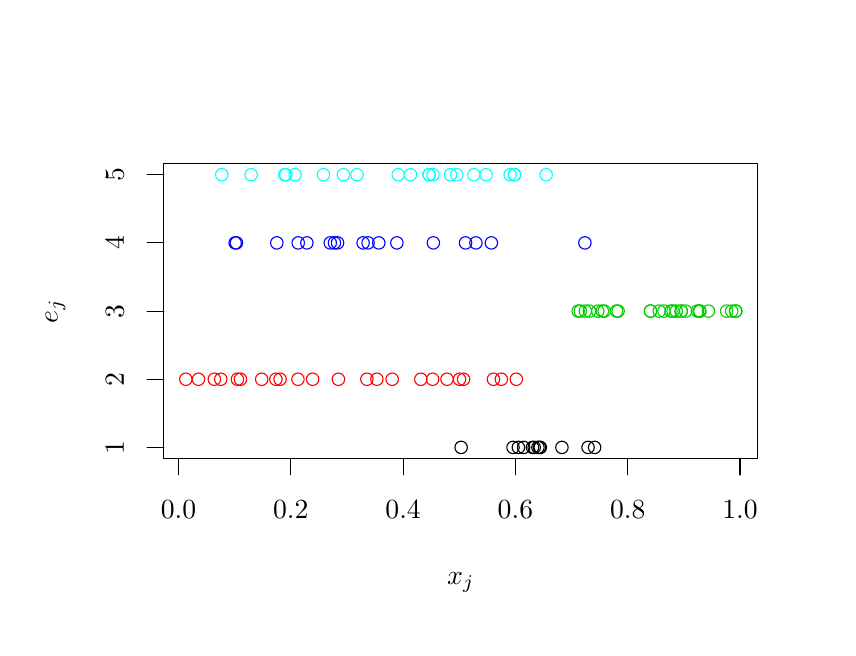
\begin{tikzpicture}[x=1pt,y=1pt]
\definecolor{fillColor}{RGB}{255,255,255}
\path[use as bounding box,fill=fillColor,fill opacity=0.00] (0,0) rectangle (289.08,216.81);
\begin{scope}
\path[clip] ( 49.20, 61.20) rectangle (263.88,167.61);
\definecolor{drawColor}{RGB}{0,255,255}

\path[draw=drawColor,line width= 0.4pt,line join=round,line cap=round] (187.35,163.67) circle (  2.25);
\definecolor{drawColor}{RGB}{255,0,0}

\path[draw=drawColor,line width= 0.4pt,line join=round,line cap=round] (126.17, 89.77) circle (  2.25);
\definecolor{drawColor}{RGB}{0,0,255}

\path[draw=drawColor,line width= 0.4pt,line join=round,line cap=round] (109.34,139.04) circle (  2.25);
\definecolor{drawColor}{RGB}{0,205,0}

\path[draw=drawColor,line width= 0.4pt,line join=round,line cap=round] (255.93,114.40) circle (  2.25);
\definecolor{drawColor}{RGB}{0,0,0}

\path[draw=drawColor,line width= 0.4pt,line join=round,line cap=round] (183.04, 65.14) circle (  2.25);
\definecolor{drawColor}{RGB}{0,0,255}

\path[draw=drawColor,line width= 0.4pt,line join=round,line cap=round] ( 97.76,139.04) circle (  2.25);
\definecolor{drawColor}{RGB}{0,255,255}

\path[draw=drawColor,line width= 0.4pt,line join=round,line cap=round] ( 80.75,163.67) circle (  2.25);
\definecolor{drawColor}{RGB}{255,0,0}

\path[draw=drawColor,line width= 0.4pt,line join=round,line cap=round] (151.52, 89.77) circle (  2.25);
\definecolor{drawColor}{RGB}{0,205,0}

\path[draw=drawColor,line width= 0.4pt,line join=round,line cap=round] (242.01,114.40) circle (  2.25);
\definecolor{drawColor}{RGB}{0,255,255}

\path[draw=drawColor,line width= 0.4pt,line join=round,line cap=round] (176.00,163.67) circle (  2.25);
\definecolor{drawColor}{RGB}{0,205,0}

\path[draw=drawColor,line width= 0.4pt,line join=round,line cap=round] (252.58,114.40) circle (  2.25);

\path[draw=drawColor,line width= 0.4pt,line join=round,line cap=round] (202.99,114.40) circle (  2.25);
\definecolor{drawColor}{RGB}{0,0,255}

\path[draw=drawColor,line width= 0.4pt,line join=round,line cap=round] (126.88,139.04) circle (  2.25);
\definecolor{drawColor}{RGB}{255,0,0}

\path[draw=drawColor,line width= 0.4pt,line join=round,line cap=round] (142.05, 89.77) circle (  2.25);

\path[draw=drawColor,line width= 0.4pt,line join=round,line cap=round] ( 84.57, 89.77) circle (  2.25);

\path[draw=drawColor,line width= 0.4pt,line join=round,line cap=round] ( 57.15, 89.77) circle (  2.25);
\definecolor{drawColor}{RGB}{0,205,0}

\path[draw=drawColor,line width= 0.4pt,line join=round,line cap=round] (199.70,114.40) circle (  2.25);
\definecolor{drawColor}{RGB}{0,0,255}

\path[draw=drawColor,line width= 0.4pt,line join=round,line cap=round] ( 75.44,139.04) circle (  2.25);
\definecolor{drawColor}{RGB}{0,255,255}

\path[draw=drawColor,line width= 0.4pt,line join=round,line cap=round] (145.06,163.67) circle (  2.25);
\definecolor{drawColor}{RGB}{0,0,0}

\path[draw=drawColor,line width= 0.4pt,line join=round,line cap=round] (184.38, 65.14) circle (  2.25);
\definecolor{drawColor}{RGB}{0,205,0}

\path[draw=drawColor,line width= 0.4pt,line join=round,line cap=round] (255.76,114.40) circle (  2.25);
\definecolor{drawColor}{RGB}{0,255,255}

\path[draw=drawColor,line width= 0.4pt,line join=round,line cap=round] (155.06,163.67) circle (  2.25);

\path[draw=drawColor,line width= 0.4pt,line join=round,line cap=round] (152.78,163.67) circle (  2.25);
\definecolor{drawColor}{RGB}{255,0,0}

\path[draw=drawColor,line width= 0.4pt,line join=round,line cap=round] ( 89.69, 89.77) circle (  2.25);
\definecolor{drawColor}{RGB}{0,205,0}

\path[draw=drawColor,line width= 0.4pt,line join=round,line cap=round] (207.66,114.40) circle (  2.25);
\definecolor{drawColor}{RGB}{0,0,255}

\path[draw=drawColor,line width= 0.4pt,line join=round,line cap=round] (146.60,139.04) circle (  2.25);

\path[draw=drawColor,line width= 0.4pt,line join=round,line cap=round] (158.22,139.04) circle (  2.25);
\definecolor{drawColor}{RGB}{0,255,255}

\path[draw=drawColor,line width= 0.4pt,line join=round,line cap=round] ( 96.61,163.67) circle (  2.25);
\definecolor{drawColor}{RGB}{0,0,255}

\path[draw=drawColor,line width= 0.4pt,line join=round,line cap=round] (100.90,139.04) circle (  2.25);
\definecolor{drawColor}{RGB}{0,0,0}

\path[draw=drawColor,line width= 0.4pt,line join=round,line cap=round] (175.38, 65.14) circle (  2.25);
\definecolor{drawColor}{RGB}{255,0,0}

\path[draw=drawColor,line width= 0.4pt,line join=round,line cap=round] (171.15, 89.77) circle (  2.25);
\definecolor{drawColor}{RGB}{0,255,255}

\path[draw=drawColor,line width= 0.4pt,line join=round,line cap=round] ( 70.14,163.67) circle (  2.25);
\definecolor{drawColor}{RGB}{255,0,0}

\path[draw=drawColor,line width= 0.4pt,line join=round,line cap=round] ( 61.71, 89.77) circle (  2.25);
\definecolor{drawColor}{RGB}{0,0,0}

\path[draw=drawColor,line width= 0.4pt,line join=round,line cap=round] (184.93, 65.14) circle (  2.25);
\definecolor{drawColor}{RGB}{0,205,0}

\path[draw=drawColor,line width= 0.4pt,line join=round,line cap=round] (242.93,114.40) circle (  2.25);
\definecolor{drawColor}{RGB}{0,255,255}

\path[draw=drawColor,line width= 0.4pt,line join=round,line cap=round] (175.86,163.67) circle (  2.25);
\definecolor{drawColor}{RGB}{255,0,0}

\path[draw=drawColor,line width= 0.4pt,line join=round,line cap=round] (168.31, 89.77) circle (  2.25);
\definecolor{drawColor}{RGB}{0,255,255}

\path[draw=drawColor,line width= 0.4pt,line join=round,line cap=round] (161.24,163.67) circle (  2.25);
\definecolor{drawColor}{RGB}{0,205,0}

\path[draw=drawColor,line width= 0.4pt,line join=round,line cap=round] (254.39,114.40) circle (  2.25);
\definecolor{drawColor}{RGB}{255,0,0}

\path[draw=drawColor,line width= 0.4pt,line join=round,line cap=round] (157.51, 89.77) circle (  2.25);
\definecolor{drawColor}{RGB}{0,0,0}

\path[draw=drawColor,line width= 0.4pt,line join=round,line cap=round] (193.05, 65.14) circle (  2.25);
\definecolor{drawColor}{RGB}{255,0,0}

\path[draw=drawColor,line width= 0.4pt,line join=round,line cap=round] (176.56, 89.77) circle (  2.25);

\path[draw=drawColor,line width= 0.4pt,line join=round,line cap=round] (102.97, 89.77) circle (  2.25);
\definecolor{drawColor}{RGB}{0,255,255}

\path[draw=drawColor,line width= 0.4pt,line join=round,line cap=round] (106.88,163.67) circle (  2.25);
\definecolor{drawColor}{RGB}{0,0,0}

\path[draw=drawColor,line width= 0.4pt,line join=round,line cap=round] (202.49, 65.14) circle (  2.25);
\definecolor{drawColor}{RGB}{255,0,0}

\path[draw=drawColor,line width= 0.4pt,line join=round,line cap=round] (146.33, 89.77) circle (  2.25);
\definecolor{drawColor}{RGB}{0,0,255}

\path[draw=drawColor,line width= 0.4pt,line join=round,line cap=round] ( 90.03,139.04) circle (  2.25);
\definecolor{drawColor}{RGB}{0,205,0}

\path[draw=drawColor,line width= 0.4pt,line join=round,line cap=round] (206.01,114.40) circle (  2.25);
\definecolor{drawColor}{RGB}{255,0,0}

\path[draw=drawColor,line width= 0.4pt,line join=round,line cap=round] ( 75.80, 89.77) circle (  2.25);
\definecolor{drawColor}{RGB}{0,205,0}

\path[draw=drawColor,line width= 0.4pt,line join=round,line cap=round] (229.93,114.40) circle (  2.25);
\definecolor{drawColor}{RGB}{0,0,0}

\path[draw=drawColor,line width= 0.4pt,line join=round,line cap=round] (179.22, 65.14) circle (  2.25);
\definecolor{drawColor}{RGB}{0,0,255}

\path[draw=drawColor,line width= 0.4pt,line join=round,line cap=round] (167.55,139.04) circle (  2.25);

\path[draw=drawColor,line width= 0.4pt,line join=round,line cap=round] (121.21,139.04) circle (  2.25);
\definecolor{drawColor}{RGB}{0,255,255}

\path[draw=drawColor,line width= 0.4pt,line join=round,line cap=round] (146.45,163.67) circle (  2.25);
\definecolor{drawColor}{RGB}{255,0,0}

\path[draw=drawColor,line width= 0.4pt,line join=round,line cap=round] (156.04, 89.77) circle (  2.25);

\path[draw=drawColor,line width= 0.4pt,line join=round,line cap=round] ( 91.20, 89.77) circle (  2.25);
\definecolor{drawColor}{RGB}{0,0,255}

\path[draw=drawColor,line width= 0.4pt,line join=round,line cap=round] (161.97,139.04) circle (  2.25);
\definecolor{drawColor}{RGB}{255,0,0}

\path[draw=drawColor,line width= 0.4pt,line join=round,line cap=round] ( 69.77, 89.77) circle (  2.25);
\definecolor{drawColor}{RGB}{0,0,255}

\path[draw=drawColor,line width= 0.4pt,line join=round,line cap=round] (110.86,139.04) circle (  2.25);
\definecolor{drawColor}{RGB}{255,0,0}

\path[draw=drawColor,line width= 0.4pt,line join=round,line cap=round] ( 97.66, 89.77) circle (  2.25);

\path[draw=drawColor,line width= 0.4pt,line join=round,line cap=round] (112.29, 89.77) circle (  2.25);
\definecolor{drawColor}{RGB}{0,205,0}

\path[draw=drawColor,line width= 0.4pt,line join=round,line cap=round] (236.13,114.40) circle (  2.25);
\definecolor{drawColor}{RGB}{0,255,255}

\path[draw=drawColor,line width= 0.4pt,line join=round,line cap=round] (145.05,163.67) circle (  2.25);
\definecolor{drawColor}{RGB}{0,205,0}

\path[draw=drawColor,line width= 0.4pt,line join=round,line cap=round] (212.77,114.40) circle (  2.25);

\path[draw=drawColor,line width= 0.4pt,line join=round,line cap=round] (233.19,114.40) circle (  2.25);
\definecolor{drawColor}{RGB}{0,255,255}

\path[draw=drawColor,line width= 0.4pt,line join=round,line cap=round] (138.33,163.67) circle (  2.25);
\definecolor{drawColor}{RGB}{255,0,0}

\path[draw=drawColor,line width= 0.4pt,line join=round,line cap=round] ( 67.45, 89.77) circle (  2.25);

\path[draw=drawColor,line width= 0.4pt,line join=round,line cap=round] (122.57, 89.77) circle (  2.25);
\definecolor{drawColor}{RGB}{0,0,255}

\path[draw=drawColor,line width= 0.4pt,line join=round,line cap=round] (201.35,139.04) circle (  2.25);

\path[draw=drawColor,line width= 0.4pt,line join=round,line cap=round] (123.00,139.04) circle (  2.25);
\definecolor{drawColor}{RGB}{0,0,0}

\path[draw=drawColor,line width= 0.4pt,line join=round,line cap=round] (182.42, 65.14) circle (  2.25);
\definecolor{drawColor}{RGB}{0,205,0}

\path[draw=drawColor,line width= 0.4pt,line join=round,line cap=round] (225.07,114.40) circle (  2.25);

\path[draw=drawColor,line width= 0.4pt,line join=round,line cap=round] (228.22,114.40) circle (  2.25);
\definecolor{drawColor}{RGB}{0,255,255}

\path[draw=drawColor,line width= 0.4pt,line join=round,line cap=round] (133.91,163.67) circle (  2.25);
\definecolor{drawColor}{RGB}{255,0,0}

\path[draw=drawColor,line width= 0.4pt,line join=round,line cap=round] (131.71, 89.77) circle (  2.25);
\definecolor{drawColor}{RGB}{0,205,0}

\path[draw=drawColor,line width= 0.4pt,line join=round,line cap=round] (236.20,114.40) circle (  2.25);
\definecolor{drawColor}{RGB}{0,0,0}

\path[draw=drawColor,line width= 0.4pt,line join=round,line cap=round] (185.24, 65.14) circle (  2.25);

\path[draw=drawColor,line width= 0.4pt,line join=round,line cap=round] (204.87, 65.14) circle (  2.25);

\path[draw=drawColor,line width= 0.4pt,line join=round,line cap=round] (177.32, 65.14) circle (  2.25);
\definecolor{drawColor}{RGB}{0,205,0}

\path[draw=drawColor,line width= 0.4pt,line join=round,line cap=round] (237.75,114.40) circle (  2.25);
\definecolor{drawColor}{RGB}{0,255,255}

\path[draw=drawColor,line width= 0.4pt,line join=round,line cap=round] (114.10,163.67) circle (  2.25);

\path[draw=drawColor,line width= 0.4pt,line join=round,line cap=round] ( 93.31,163.67) circle (  2.25);
\definecolor{drawColor}{RGB}{0,205,0}

\path[draw=drawColor,line width= 0.4pt,line join=round,line cap=round] (234.37,114.40) circle (  2.25);
\definecolor{drawColor}{RGB}{0,0,0}

\path[draw=drawColor,line width= 0.4pt,line join=round,line cap=round] (156.63, 65.14) circle (  2.25);
\definecolor{drawColor}{RGB}{0,205,0}

\path[draw=drawColor,line width= 0.4pt,line join=round,line cap=round] (232.47,114.40) circle (  2.25);
\definecolor{drawColor}{RGB}{0,255,255}

\path[draw=drawColor,line width= 0.4pt,line join=round,line cap=round] ( 92.89,163.67) circle (  2.25);
\definecolor{drawColor}{RGB}{0,205,0}

\path[draw=drawColor,line width= 0.4pt,line join=round,line cap=round] (208.33,114.40) circle (  2.25);

\path[draw=drawColor,line width= 0.4pt,line join=round,line cap=round] (201.51,114.40) circle (  2.25);

\path[draw=drawColor,line width= 0.4pt,line join=round,line cap=round] (245.99,114.40) circle (  2.25);
\definecolor{drawColor}{RGB}{0,255,255}

\path[draw=drawColor,line width= 0.4pt,line join=round,line cap=round] (165.62,163.67) circle (  2.25);
\definecolor{drawColor}{RGB}{0,205,0}

\path[draw=drawColor,line width= 0.4pt,line join=round,line cap=round] (198.92,114.40) circle (  2.25);
\definecolor{drawColor}{RGB}{0,0,255}

\path[draw=drawColor,line width= 0.4pt,line join=round,line cap=round] (133.41,139.04) circle (  2.25);

\path[draw=drawColor,line width= 0.4pt,line join=round,line cap=round] ( 74.97,139.04) circle (  2.25);
\definecolor{drawColor}{RGB}{0,205,0}

\path[draw=drawColor,line width= 0.4pt,line join=round,line cap=round] (242.66,114.40) circle (  2.25);
\definecolor{drawColor}{RGB}{0,0,255}

\path[draw=drawColor,line width= 0.4pt,line join=round,line cap=round] (111.97,139.04) circle (  2.25);
\definecolor{drawColor}{RGB}{0,255,255}

\path[draw=drawColor,line width= 0.4pt,line join=round,line cap=round] (174.33,163.67) circle (  2.25);
\definecolor{drawColor}{RGB}{255,0,0}

\path[draw=drawColor,line width= 0.4pt,line join=round,line cap=round] ( 76.89, 89.77) circle (  2.25);
\definecolor{drawColor}{RGB}{0,205,0}

\path[draw=drawColor,line width= 0.4pt,line join=round,line cap=round] (225.05,114.40) circle (  2.25);
\definecolor{drawColor}{RGB}{0,255,255}

\path[draw=drawColor,line width= 0.4pt,line join=round,line cap=round] (119.02,163.67) circle (  2.25);
\definecolor{drawColor}{RGB}{0,205,0}

\path[draw=drawColor,line width= 0.4pt,line join=round,line cap=round] (213.35,114.40) circle (  2.25);
\end{scope}
\begin{scope}
\path[clip] (  0.00,  0.00) rectangle (289.08,216.81);
\definecolor{drawColor}{RGB}{0,0,0}

\path[draw=drawColor,line width= 0.4pt,line join=round,line cap=round] ( 54.50, 61.20) -- (257.41, 61.20);

\path[draw=drawColor,line width= 0.4pt,line join=round,line cap=round] ( 54.50, 61.20) -- ( 54.50, 55.20);

\path[draw=drawColor,line width= 0.4pt,line join=round,line cap=round] ( 95.08, 61.20) -- ( 95.08, 55.20);

\path[draw=drawColor,line width= 0.4pt,line join=round,line cap=round] (135.66, 61.20) -- (135.66, 55.20);

\path[draw=drawColor,line width= 0.4pt,line join=round,line cap=round] (176.25, 61.20) -- (176.25, 55.20);

\path[draw=drawColor,line width= 0.4pt,line join=round,line cap=round] (216.83, 61.20) -- (216.83, 55.20);

\path[draw=drawColor,line width= 0.4pt,line join=round,line cap=round] (257.41, 61.20) -- (257.41, 55.20);

\node[text=drawColor,anchor=base,inner sep=0pt, outer sep=0pt, scale=  1.00] at ( 54.50, 39.60) {0.0};

\node[text=drawColor,anchor=base,inner sep=0pt, outer sep=0pt, scale=  1.00] at ( 95.08, 39.60) {0.2};

\node[text=drawColor,anchor=base,inner sep=0pt, outer sep=0pt, scale=  1.00] at (135.66, 39.60) {0.4};

\node[text=drawColor,anchor=base,inner sep=0pt, outer sep=0pt, scale=  1.00] at (176.25, 39.60) {0.6};

\node[text=drawColor,anchor=base,inner sep=0pt, outer sep=0pt, scale=  1.00] at (216.83, 39.60) {0.8};

\node[text=drawColor,anchor=base,inner sep=0pt, outer sep=0pt, scale=  1.00] at (257.41, 39.60) {1.0};

\path[draw=drawColor,line width= 0.4pt,line join=round,line cap=round] ( 49.20, 65.14) -- ( 49.20,163.67);

\path[draw=drawColor,line width= 0.4pt,line join=round,line cap=round] ( 49.20, 65.14) -- ( 43.20, 65.14);

\path[draw=drawColor,line width= 0.4pt,line join=round,line cap=round] ( 49.20, 89.77) -- ( 43.20, 89.77);

\path[draw=drawColor,line width= 0.4pt,line join=round,line cap=round] ( 49.20,114.40) -- ( 43.20,114.40);

\path[draw=drawColor,line width= 0.4pt,line join=round,line cap=round] ( 49.20,139.04) -- ( 43.20,139.04);

\path[draw=drawColor,line width= 0.4pt,line join=round,line cap=round] ( 49.20,163.67) -- ( 43.20,163.67);

\node[text=drawColor,rotate= 90.00,anchor=base,inner sep=0pt, outer sep=0pt, scale=  1.00] at ( 34.80, 65.14) {1};

\node[text=drawColor,rotate= 90.00,anchor=base,inner sep=0pt, outer sep=0pt, scale=  1.00] at ( 34.80, 89.77) {2};

\node[text=drawColor,rotate= 90.00,anchor=base,inner sep=0pt, outer sep=0pt, scale=  1.00] at ( 34.80,114.40) {3};

\node[text=drawColor,rotate= 90.00,anchor=base,inner sep=0pt, outer sep=0pt, scale=  1.00] at ( 34.80,139.04) {4};

\node[text=drawColor,rotate= 90.00,anchor=base,inner sep=0pt, outer sep=0pt, scale=  1.00] at ( 34.80,163.67) {5};

\path[draw=drawColor,line width= 0.4pt,line join=round,line cap=round] ( 49.20, 61.20) --
	(263.88, 61.20) --
	(263.88,167.61) --
	( 49.20,167.61) --
	( 49.20, 61.20);
\end{scope}
\begin{scope}
\path[clip] (  0.00,  0.00) rectangle (289.08,216.81);
\definecolor{drawColor}{RGB}{0,0,0}

\node[text=drawColor,anchor=base,inner sep=0pt, outer sep=0pt, scale=  1.00] at (156.54, 15.60) {$x_j$};

\node[text=drawColor,rotate= 90.00,anchor=base,inner sep=0pt, outer sep=0pt, scale=  1.00] at ( 10.80,114.41) {$e_j$};
\end{scope}
\end{tikzpicture}
